\documentclass[american,]{article}
\usepackage{lmodern}
\usepackage{amssymb,amsmath}
\usepackage{ifxetex,ifluatex}
\usepackage{pdfpages}
\usepackage{appendix}
\usepackage{fixltx2e} % provides \textsubscript
\ifnum 0\ifxetex 1\fi\ifluatex 1\fi=0 % if pdftex
  \usepackage[T1]{fontenc}
  \usepackage[utf8]{inputenc}
\else % if luatex or xelatex
  \ifxetex
    \usepackage{mathspec}
  \else
    \usepackage{fontspec}
  \fi
  \defaultfontfeatures{Ligatures=TeX,Scale=MatchLowercase}
\fi
% use upquote if available, for straight quotes in verbatim environments
\IfFileExists{upquote.sty}{\usepackage{upquote}}{}
% use microtype if available
\IfFileExists{microtype.sty}{%
\usepackage{microtype}
\UseMicrotypeSet[protrusion]{basicmath} % disable protrusion for tt fonts
}{}
\usepackage[margin=1in]{geometry}
\usepackage{hyperref}
\hypersetup{unicode=true,
            pdftitle={Predicting Quarterback Fantasy Score},
            pdfauthor={Kevin Thompson, Sean Kennedy, and Sachin Chavan},
            pdfborder={0 0 0},
            breaklinks=true}
\urlstyle{same}  % don't use monospace font for urls
\ifnum 0\ifxetex 1\fi\ifluatex 1\fi=0 % if pdftex
  \usepackage[shorthands=off,main=american]{babel}
\else
  \usepackage{polyglossia}
  \setmainlanguage[variant=american]{english}
\fi
\usepackage{natbib}
\bibliographystyle{apalike}
\usepackage{longtable,booktabs}
\usepackage{graphicx,grffile}
\makeatletter
\def\maxwidth{\ifdim\Gin@nat@width>\linewidth\linewidth\else\Gin@nat@width\fi}
\def\maxheight{\ifdim\Gin@nat@height>\textheight\textheight\else\Gin@nat@height\fi}
\makeatother
% Scale images if necessary, so that they will not overflow the page
% margins by default, and it is still possible to overwrite the defaults
% using explicit options in \includegraphics[width, height, ...]{}
\setkeys{Gin}{width=\maxwidth,height=\maxheight,keepaspectratio}
\IfFileExists{parskip.sty}{%
\usepackage{parskip}
}{% else
\setlength{\parindent}{0pt}
\setlength{\parskip}{6pt plus 2pt minus 1pt}
}
\setlength{\emergencystretch}{3em}  % prevent overfull lines
\providecommand{\tightlist}{%
  \setlength{\itemsep}{0pt}\setlength{\parskip}{0pt}}
\setcounter{secnumdepth}{5}
% Redefines (sub)paragraphs to behave more like sections
\ifx\paragraph\undefined\else
\let\oldparagraph\paragraph
\renewcommand{\paragraph}[1]{\oldparagraph{#1}\mbox{}}
\fi
\ifx\subparagraph\undefined\else
\let\oldsubparagraph\subparagraph
\renewcommand{\subparagraph}[1]{\oldsubparagraph{#1}\mbox{}}
\fi

%%% Use protect on footnotes to avoid problems with footnotes in titles
\let\rmarkdownfootnote\footnote%
\def\footnote{\protect\rmarkdownfootnote}

%%% Change title format to be more compact
\usepackage{titling}

% Create subtitle command for use in maketitle
\providecommand{\subtitle}[1]{
  \posttitle{
    \begin{center}\large#1\end{center}
    }
}

\setlength{\droptitle}{-2em}

  \title{Predicting Quarterback Fantasy Score}
    \pretitle{\vspace{\droptitle}\centering\huge}
  \posttitle{\par}
    \author{Kevin Thompson, Sean Kennedy, and Sachin Chavan}
    \preauthor{\centering\large\emph}
  \postauthor{\par}
      \predate{\centering\large\emph}
  \postdate{\par}
    \date{Data Science Program, Southern Methodist University, USA \break"}

\usepackage{amsmath}
\usepackage[utf8]{inputenc}
\usepackage[T1]{fontenc}
\usepackage{setspace}
\usepackage{hyperref}
\onehalfspacing
\setcitestyle{round}
\newcommand\numberthis{\addtocounter{equation}{1}\tag{\theequation}}
\begin{document}
\maketitle
\begin{abstract}
Hype.
\end{abstract}

\section{Introduction}\label{introduction}

Fantasy sports are a big business. Generating nearly 7 billion dollars
annually (cite) and with approximately 60 million players in the
US/Canada (cite), fantasy sports -- particularly football -- have become
as big as the sports that they mimic. Players can compete head to head
in leagues across a wide range of providers (Yahoo, CBS, ESPN,
DraftKings, DraftStreet etc) -- each with their own rulesets and stakes.
Some are just friendly leagues set up between friends or coworkers, no
real stakes other than bragging rights, others have significant monetary
rewards for those that can get to the top of the leaderboard.

The explosion of weekly leagues over the course of the last few years
has seen an already huge business get even larger. In the weekly cash
leagues -- each player is given a budget and drafts a completely new
team every week. Each draft site uses a predictive model to set player
salaries based on the number of points the model predicts that player to
score. Budget constraints make it impossible to simply select the
players that are predicted to score the most points -- hence having a
predictive model for which players will generate the best return on
investment would be a huge advantage. In the following analysis we will
attempt to build position specific models that can accurately predict
the number of points a given NFL player is likely to score in a given
week.

\section{Data Description}\label{data-description}

The \textbf{fantasydata.com} is leading sports data company, providing real-time post games feeds across all major sports to both fantasy and other companies. For this exercise NFL data was retrived through API calls for predicting quarterback's performance in next match by estimating fantasypoints. For model building 17 weeks of data was obtained for around 56 players for season 2017. This dataset contains 453 quarterabck's observations from 17 matches and 512 observations of opponent's team. These observations contains 13 explanatory variables for quarterback and 18 derived from defensive statistics i.e. from opponent team. For the first analysis in this paper, we have focused on predicting Fantasypoints in the next match based on data available till current game. Since this is weekly data for individual player, The second analysis expands this anlalys to building time series model to forecast performance in next matches. More information on the details can be found in the analyses that follow. 

\section{Exploratory Analysis}\label{exploratory-analysis}

Data was retrived from real-time post games feed made available by fantasydata website. Quarterback with 453 observations for about 56 players and defensive statistics with 512 observations was analyzed for missing information. Data appeared to be clean. Section 6 of Appendix-I shows data is clean, there are no missing values and therefore no data cleaning operation was required. This dataset contains statistics of weekly performance, All possible variables were examined during exploratory analysis and variables which found to have influence on fantasyPoints (Target Variable) were selected. Thirteen base predictors were found with linear relationship with FantasyPoints and 18 are derived from defensive statistics. Scatterplots of base and derived predictors have been added to section 9 of the Appendix-I. Here is the Corroleogram for base and derived predictors. 


\graphicspath{ {images/} }
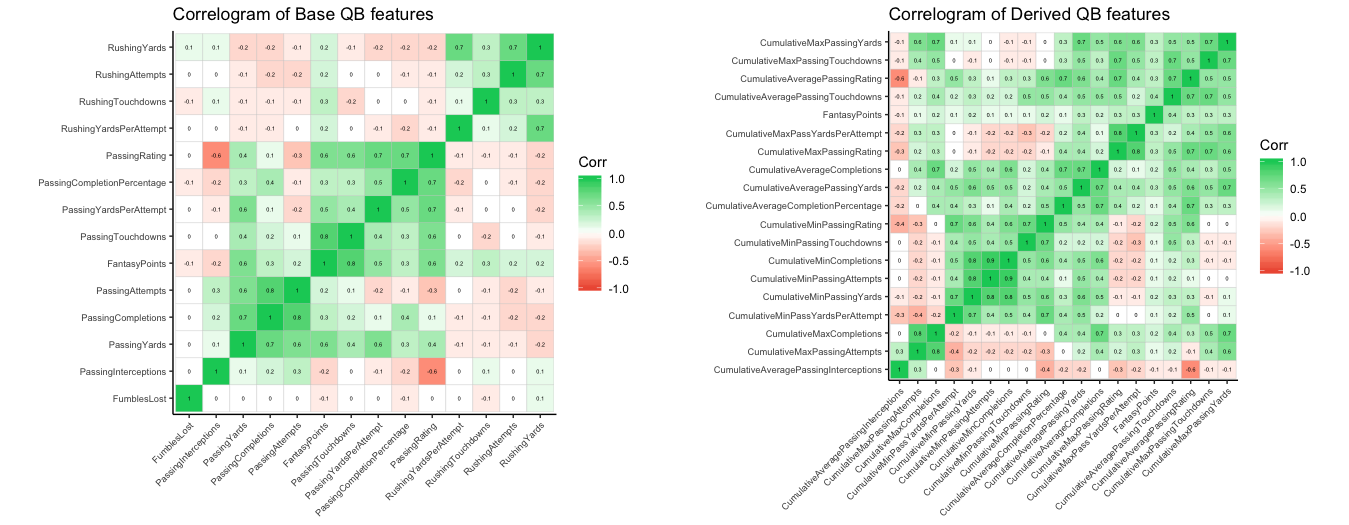
\includegraphics{img001.png}


\section{Objective One}\label{objective-one}

\subsection{Model Selection}\label{model-selection}

\subsubsection{Type of Selection}\label{type-of-selection}

Of the tools made available to us in the course, we believe that LASSO
estimation is the best option available to us. Subset selection
discretely adds and removes variables, leaving far too much room for
overfitting. While ridge regression is a great shrinkage method for many
scenarios, we believe that it is at least slightly desirable for the
coefficients of truly unnecessary variables to actually be zero so that
some true form of variable selection is occurring. We are implicitly
saying that a small set of variables are necessary to predict fantasy
scores, but the nature of football, the size of our dataset, and the
disproportionate amount of points that goes to touchdowns indicates that
this assumptions may very well be appropriate.

\subsubsection{Assumption-Checking}\label{assumption-checking}

The LASSO model is a linear model and thus assumes that there is a
linear relationship between the response and the parameters.
Furthermore, it is also important that the variance of the residuals is
constant across the predictors in order for our model to adequately
capture the variation in the response. Because we are not interested in
quantifying our uncertainty, we don't make any assumptions about the
distribution of the residuals.

Fit diagnostics are given in the set of plots represented in below plot.

\paragraph{Residual Plots} 
An examination of the residual plots fitted data shows a more randomized pattern for both the regular and studentized residuals.  The residual Q-Q plot shows a nice linear trend, and the residual histogram is very nearly normally distributed.
\paragraph{Influential point analysis}
only one observation stood out immediately on the Cook’s D plot, so it is necessary to examine this outlier and see what is going on.  Upon further inspection, the data point appears to be valid, so there is no good reason to exclude it from the analysis, and we can proceed with caution.
\paragraph{Linearity}
the FantasyPoints by 13 predictors do appear to be linear, as per scatterplots in section 9 of the appendix.
\paragraph{Normality}
As shown in the QQ plot. Residuals are normally distributed, it means FantasyPoints do appear to be linear with defensive variables AvgPassDefense and cumulative sum variables dervived from defensive statistics. 
\paragraph{Independence}
for Multiple linear regression, model is used to predict performance of quarterback in the next game based on today's performance taking into consideration 
oppoent't performance befor playing against them. so data is assumed to be independence.
\paragraph{Constant Variance}
Residual vs fitted plot shows random cloud which indicates there is constant variance.

\graphicspath{ {images/} }
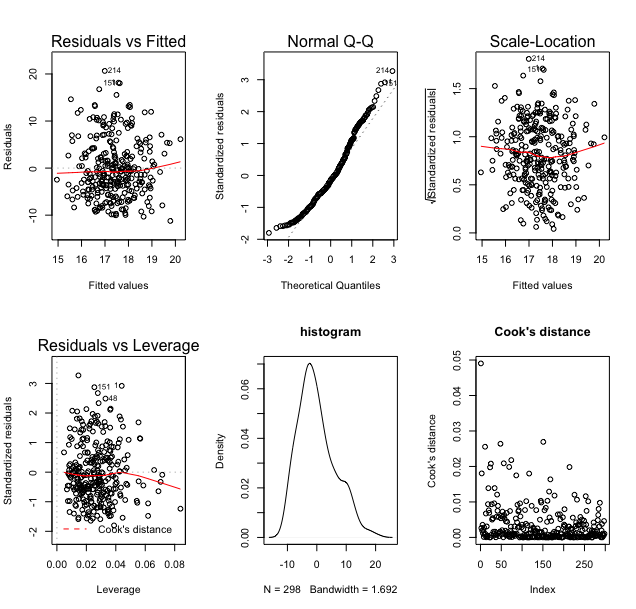
\includegraphics[width=500px,height=300px]{img002.png}

\section{Objective Two}\label{objective-two}

\renewcommand\refname{Conclusion}
\bibliography{stats2proj.bib}



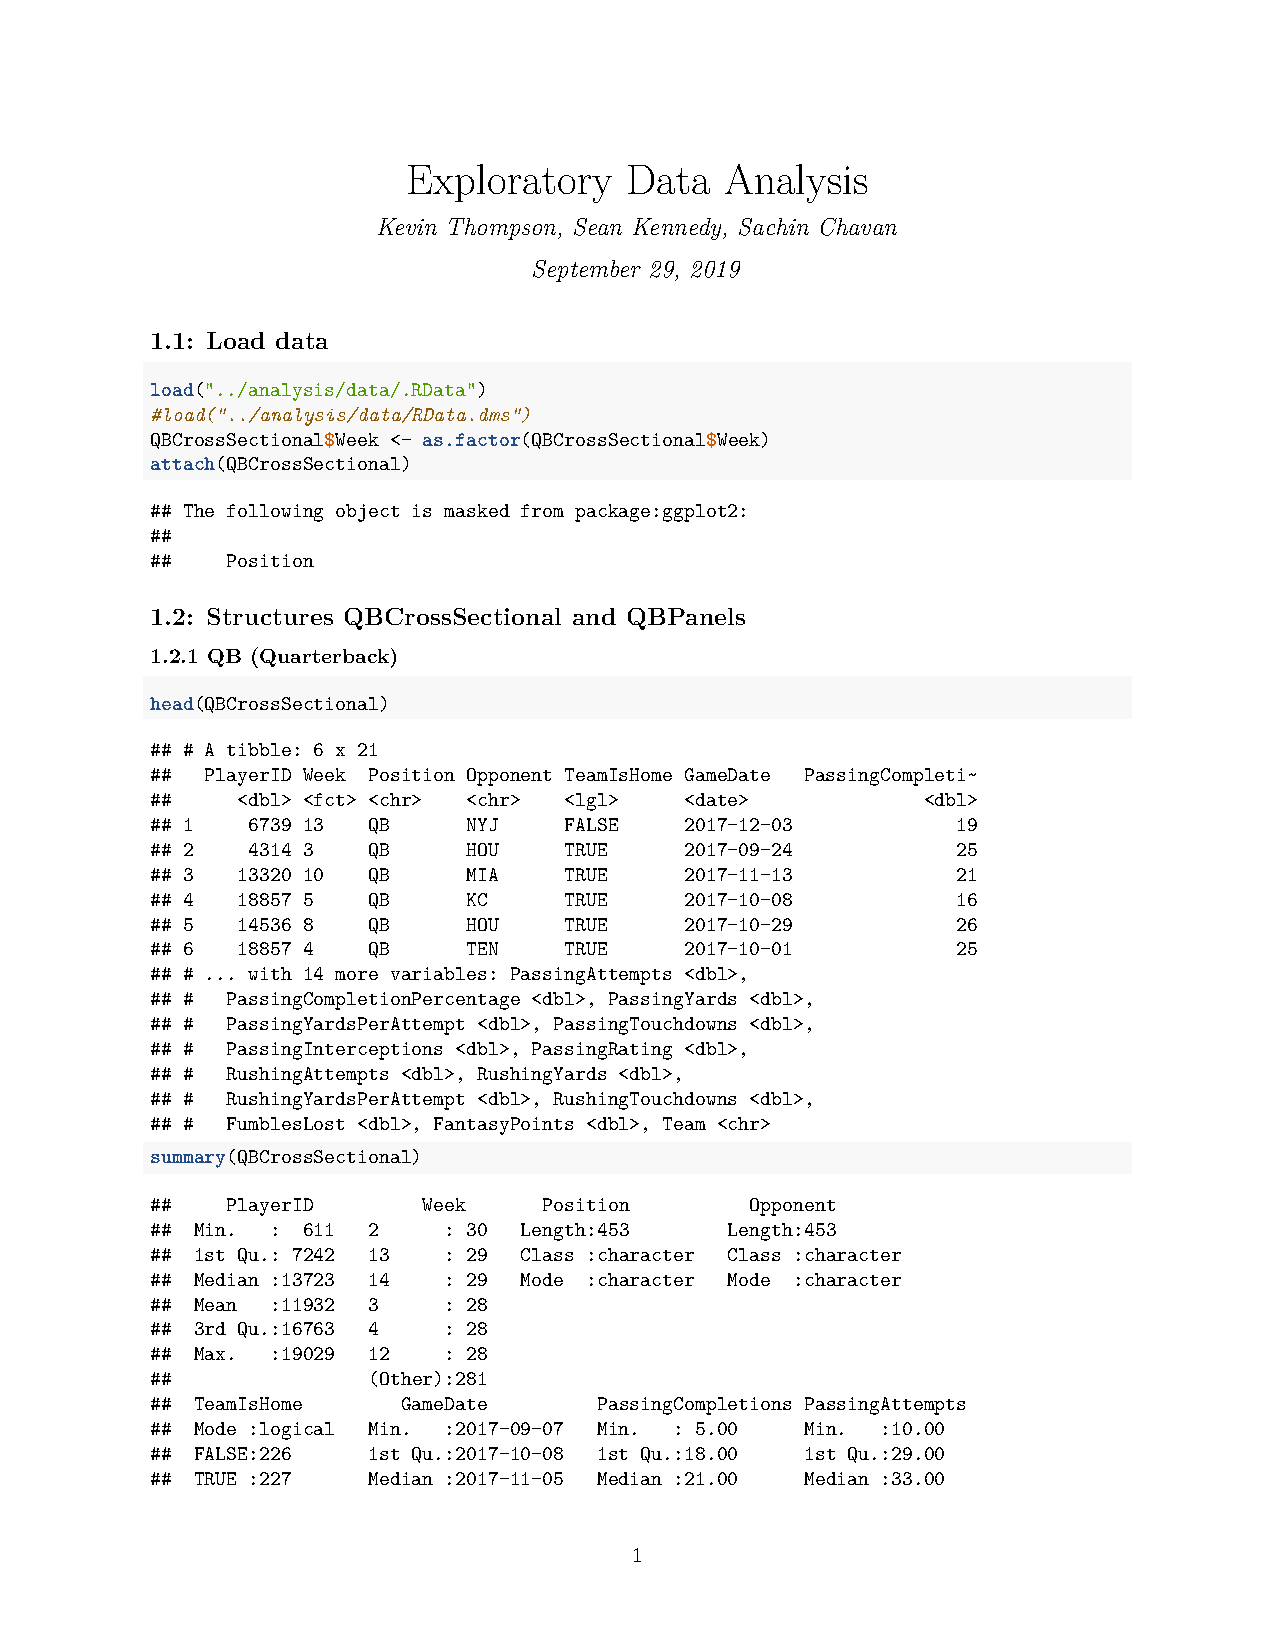
\includepdf[pages=-]{eda/eda_summary.pdf}



\end{document}
